\begin{figure}[!h]
\centering
\resizebox{\textwidth}{!}{%
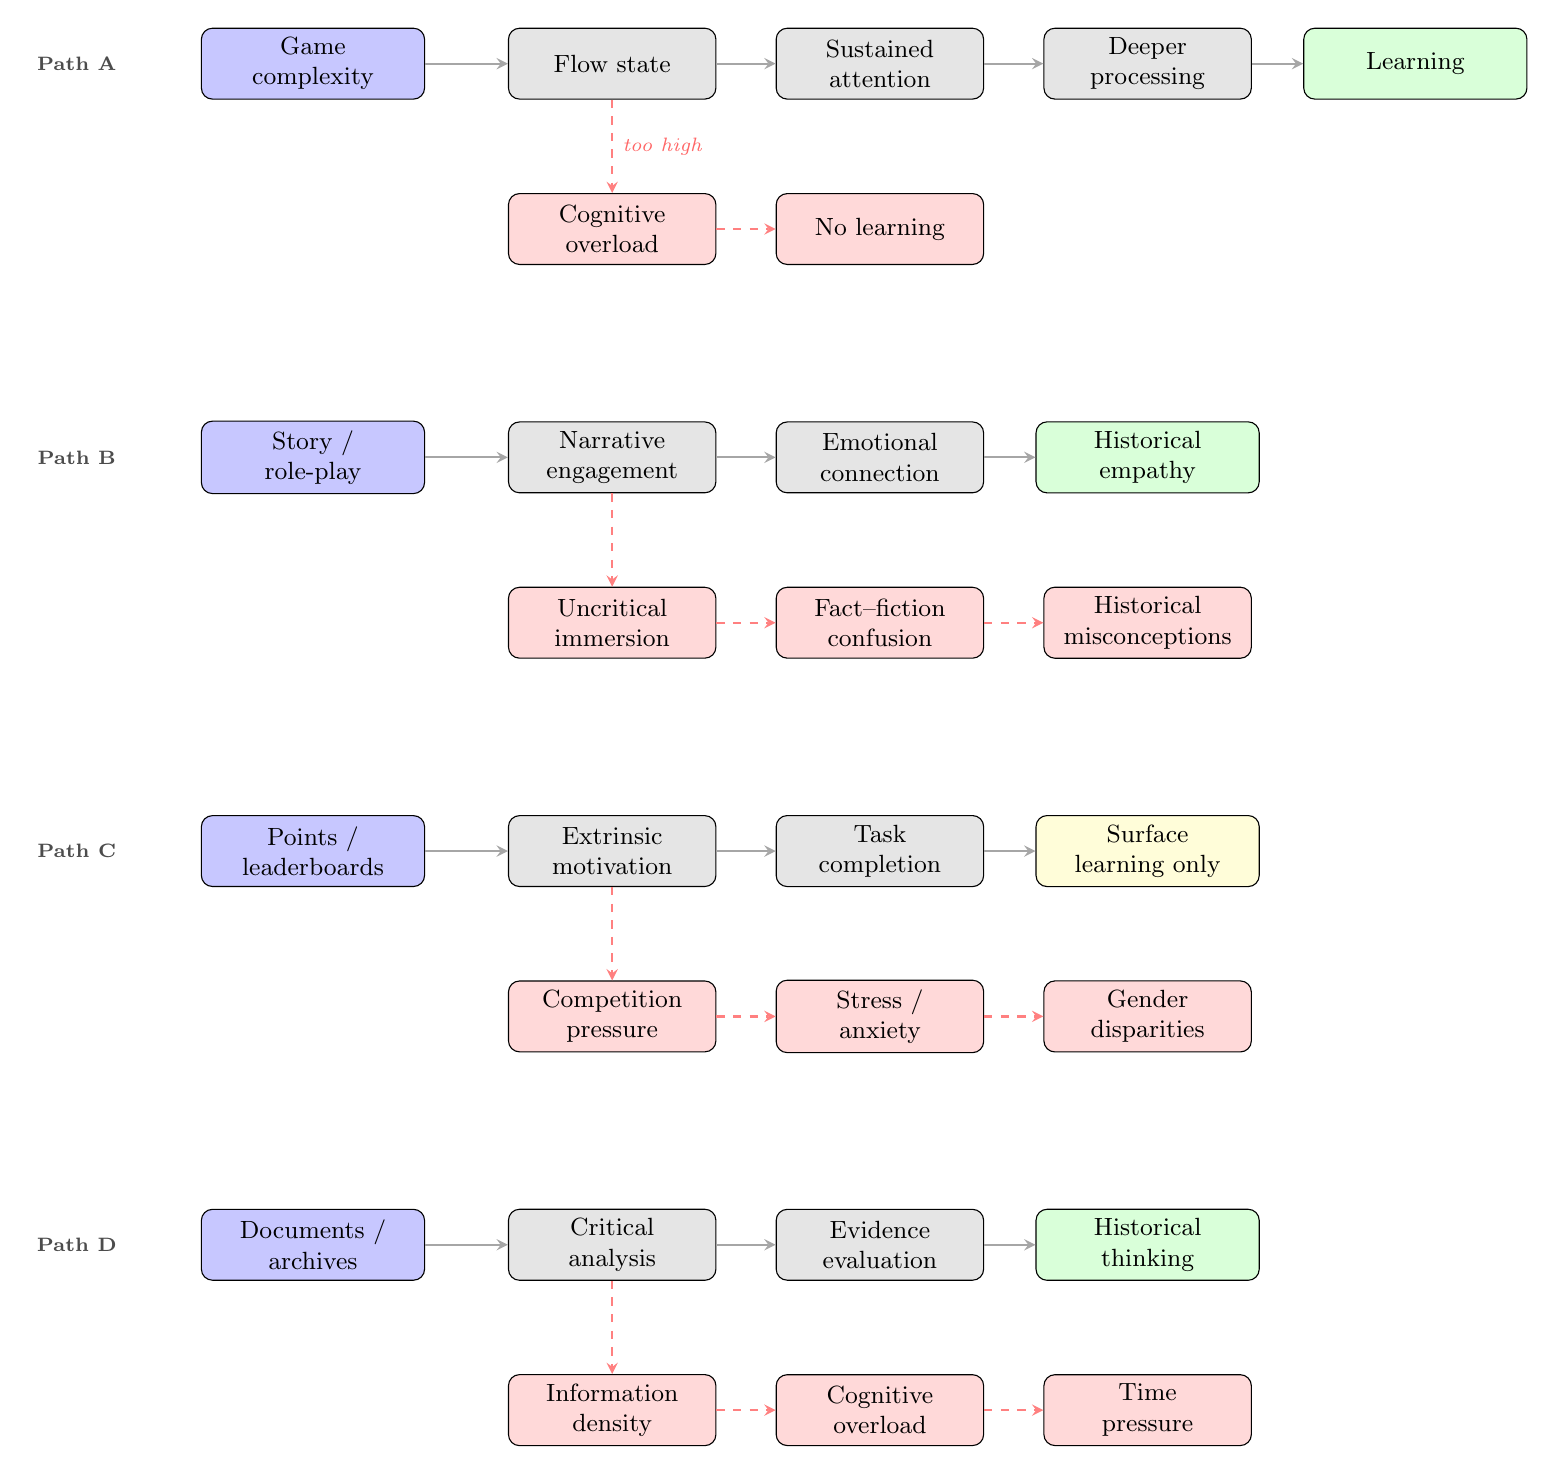
\begin{tikzpicture}[
  gamebox/.style={rectangle, draw, rounded corners=4pt, fill=blue!22,
    text width=2.6cm, minimum height=0.9cm, align=center, font=\small},
  mechbox/.style={rectangle, draw, rounded corners=4pt, fill=gray!20,
    text width=2.4cm, minimum height=0.9cm, align=center, font=\small},
  posbox/.style={rectangle, draw, rounded corners=4pt, fill=green!15,
    text width=2.6cm, minimum height=0.9cm, align=center, font=\small},
  riskbox/.style={rectangle, draw, rounded corners=4pt, fill=red!15,
    text width=2.4cm, minimum height=0.9cm, align=center, font=\small},
  pathlabel/.style={font=\scriptsize\bfseries, text=black!70},
  arr/.style={->, >=stealth, thick, draw=gray!70},
  riskarr/.style={->, >=stealth, thick, draw=red!50, dashed},
]

% Vertical spacing between pathways
\def\patha{0}
\def\pathb{-5.0}
\def\pathc{-10.0}
\def\pathd{-15.0}

% Horizontal positions
\def\xlabel{-3.0}
\def\xgame{0}
\def\xmechA{3.8}
\def\xmechB{7.2}
\def\xmechC{10.6}
\def\xout{14.0}

% ============================================================
% PATH A: Flow pathway
% ============================================================
\node[pathlabel] at (\xlabel, \patha) {Path A};

\node[gamebox] (a1) at (\xgame, \patha) {Game\\complexity};
\node[mechbox] (a2) at (\xmechA, \patha) {Flow state};
\node[mechbox] (a3) at (\xmechB, \patha) {Sustained\\attention};
\node[mechbox] (a4) at (\xmechC, \patha) {Deeper\\processing};
\node[posbox]  (a5) at (\xout, \patha) {Learning};

\draw[arr] (a1) -- (a2);
\draw[arr] (a2) -- (a3);
\draw[arr] (a3) -- (a4);
\draw[arr] (a4) -- (a5);

% Risk branch A: from a2 downward
\node[riskbox] (a2r) at (\xmechA, \patha - 2.1) {Cognitive\\overload};
\node[riskbox] (a3r) at (\xmechB, \patha - 2.1) {No learning};

\draw[riskarr] (a2.south) -- node[right, font=\scriptsize, text=red!60] {\textit{too high}} (a2r.north);
\draw[riskarr] (a2r) -- (a3r);

% ============================================================
% PATH B: Narrative pathway
% ============================================================
\node[pathlabel] at (\xlabel, \pathb) {Path B};

\node[gamebox] (b1) at (\xgame, \pathb) {Story /\\role-play};
\node[mechbox] (b2) at (\xmechA, \pathb) {Narrative\\engagement};
\node[mechbox] (b3) at (\xmechB, \pathb) {Emotional\\connection};
\node[posbox]  (b4) at (\xmechC, \pathb) {Historical\\empathy};

\draw[arr] (b1) -- (b2);
\draw[arr] (b2) -- (b3);
\draw[arr] (b3) -- (b4);

% Risk branch B: from b2 downward
\node[riskbox] (b2r) at (\xmechA, \pathb - 2.1) {Uncritical\\immersion};
\node[riskbox] (b3r) at (\xmechB, \pathb - 2.1) {Fact--fiction\\confusion};
\node[riskbox] (b4r) at (\xmechC, \pathb - 2.1) {Historical\\misconceptions};

\draw[riskarr] (b2.south) -- (b2r.north);
\draw[riskarr] (b2r) -- (b3r);
\draw[riskarr] (b3r) -- (b4r);

% ============================================================
% PATH C: Competition pathway
% ============================================================
\node[pathlabel] at (\xlabel, \pathc) {Path C};

\node[gamebox] (c1) at (\xgame, \pathc) {Points /\\leaderboards};
\node[mechbox] (c2) at (\xmechA, \pathc) {Extrinsic\\motivation};
\node[mechbox] (c3) at (\xmechB, \pathc) {Task\\completion};
\node[posbox, fill=yellow!15] (c4) at (\xmechC, \pathc) {Surface\\learning only};

\draw[arr] (c1) -- (c2);
\draw[arr] (c2) -- (c3);
\draw[arr] (c3) -- (c4);

% Risk branch C: from c2 downward
\node[riskbox] (c2r) at (\xmechA, \pathc - 2.1) {Competition\\pressure};
\node[riskbox] (c3r) at (\xmechB, \pathc - 2.1) {Stress /\\anxiety};
\node[riskbox] (c4r) at (\xmechC, \pathc - 2.1) {Gender\\disparities};

\draw[riskarr] (c2.south) -- (c2r.north);
\draw[riskarr] (c2r) -- (c3r);
\draw[riskarr] (c3r) -- (c4r);

% ============================================================
% PATH D: Source interaction pathway
% ============================================================
\node[pathlabel] at (\xlabel, \pathd) {Path D};

\node[gamebox] (d1) at (\xgame, \pathd) {Documents /\\archives};
\node[mechbox] (d2) at (\xmechA, \pathd) {Critical\\analysis};
\node[mechbox] (d3) at (\xmechB, \pathd) {Evidence\\evaluation};
\node[posbox]  (d4) at (\xmechC, \pathd) {Historical\\thinking};

\draw[arr] (d1) -- (d2);
\draw[arr] (d2) -- (d3);
\draw[arr] (d3) -- (d4);

% Risk branch D: from d2 downward
\node[riskbox] (d2r) at (\xmechA, \pathd - 2.1) {Information\\density};
\node[riskbox] (d3r) at (\xmechB, \pathd - 2.1) {Cognitive\\overload};
\node[riskbox] (d4r) at (\xmechC, \pathd - 2.1) {Time\\pressure};

\draw[riskarr] (d2.south) -- (d2r.north);
\draw[riskarr] (d2r) -- (d3r);
\draw[riskarr] (d3r) -- (d4r);

\end{tikzpicture}%
}% end resizebox
\caption{Four causal pathways from gamification elements to learning outcomes in history education. Each pathway has characteristic positive outcomes (right) and associated risks (below). Paths A, B, and D lead to deeper outcomes; Path C explains why some gamification produces engagement without learning.}
\label{fig:causal-pathways}
\end{figure}
